\documentclass[journal,12pt,twocolumn]{IEEEtran}
%
\usepackage{setspace}
\usepackage{gensymb}
\singlespacing
\usepackage[cmex10]{amsmath}
\usepackage{siunitx}
\usepackage{amsthm}

\usepackage{mathrsfs}

\usepackage{txfonts}
\usepackage{stfloats}

\usepackage{steinmetz}
\usepackage{cite}
\usepackage{cases}
\usepackage{subfig}
\usepackage{longtable}
\usepackage{multirow}
\usepackage{enumitem}
\usepackage{mathtools}
\usepackage{tikz}
\usepackage{circuitikz}
\usepackage{verbatim}
\usepackage{tfrupee}
\usepackage[breaklinks=true]{hyperref}
\usepackage{tkz-euclide} % loads  TikZ and tkz-base
\usetikzlibrary{calc,math}
\usetikzlibrary{fadings}
\usepackage{listings}
    \usepackage{color}                                            %%
    \usepackage{array}                                            %%
    \usepackage{longtable}                                        %%
    \usepackage{calc}                                             %%
    \usepackage{multirow}                                         %%
    \usepackage{hhline}                                           %%
    \usepackage{ifthen}                                           %%
  %optionally (for landscape tables embedded in another document): %%
    \usepackage{lscape}     
\usepackage{multicol}
\usepackage{chngcntr}
\DeclareMathOperator*{\Res}{Res}

\renewcommand\thesection{\arabic{section}}
\renewcommand\thesubsection{\thesection.\arabic{subsection}}
\renewcommand\thesubsubsection{\thesubsection.\arabic{subsubsection}}

\renewcommand\thesectiondis{\arabic{section}}
\renewcommand\thesubsectiondis{\thesectiondis.\arabic{subsection}}
\renewcommand\thesubsubsectiondis{\thesubsectiondis.\arabic{subsubsection}}

\hyphenation{op-tical net-works semi-conduc-tor}
\def\inputGnumericTable{}                                 %%

\lstset{
%language=C,
frame=single, 
breaklines=true,
columns=fullflexible
}
\begin{document}
%


\newtheorem{theorem}{Theorem}[section]
\newtheorem{problem}{Problem}
\newtheorem{proposition}{Proposition}[section]
\newtheorem{lemma}{Lemma}[section]
\newtheorem{corollary}[theorem]{Corollary}
\newtheorem{example}{Example}[section]
\newtheorem{definition}[problem]{Definition}
\newcommand{\BEQA}{\begin{eqnarray}}
\newcommand{\EEQA}{\end{eqnarray}}
\newcommand{\define}{\stackrel{\triangle}{=}}
\bibliographystyle{IEEEtran}
\providecommand{\mbf}{\mathbf}
\providecommand{\pr}[1]{\ensuremath{\Pr\left(#1\right)}}
\providecommand{\qfunc}[1]{\ensuremath{Q\left(#1\right)}}
\providecommand{\sbrak}[1]{\ensuremath{{}\left[#1\right]}}
\providecommand{\lsbrak}[1]{\ensuremath{{}\left[#1\right.}}
\providecommand{\rsbrak}[1]{\ensuremath{{}\left.#1\right]}}
\providecommand{\brak}[1]{\ensuremath{\left(#1\right)}}
\providecommand{\lbrak}[1]{\ensuremath{\left(#1\right.}}
\providecommand{\rbrak}[1]{\ensuremath{\left.#1\right)}}
\providecommand{\cbrak}[1]{\ensuremath{\left\{#1\right\}}}
\providecommand{\lcbrak}[1]{\ensuremath{\left\{#1\right.}}
\providecommand{\rcbrak}[1]{\ensuremath{\left.#1\right\}}}
\theoremstyle{remark}
\newtheorem{rem}{Remark}
\newcommand{\sgn}{\mathop{\mathrm{sgn}}}
\providecommand{\abs}[1]{\left\vert#1\right\vert}
\providecommand{\abs}[1]{\lvert#1\rvert} 
\providecommand{\res}[1]{\Res\displaylimits_{#1}} 
\providecommand{\norm}[1]{\left\lVert#1\right\rVert}
%\providecommand{\norm}[1]{\lVert#1\rVert}
\providecommand{\mtx}[1]{\mathbf{#1}}
\providecommand{\mean}[1]{E\left[ #1 \right]}
\providecommand{\fourier}{\overset{\mathcal{F}}{ \rightleftharpoons}}
%\providecommand{\hilbert}{\overset{\mathcal{H}}{ \rightleftharpoons}}
\providecommand{\system}{\overset{\mathcal{H}}{ \longleftrightarrow}}
	%\newcommand{\solution}[2]{\textbf{Solution:}{#1}}
\newcommand{\solution}{\noindent \textbf{Solution: }}
\newcommand{\cosec}{\,\text{cosec}\,}
\providecommand{\dec}[2]{\ensuremath{\overset{#1}{\underset{#2}{\gtrless}}}}
\newcommand{\myvec}[1]{\ensuremath{\begin{pmatrix}#1\end{pmatrix}}}
\newcommand{\mydet}[1]{\ensuremath{\begin{vmatrix}#1\end{vmatrix}}}
\numberwithin{equation}{subsection}
\makeatletter
\@addtoreset{figure}{problem}
\makeatother
\let\StandardTheFigure\thefigure
\let\vec\mathbf
\renewcommand{\thefigure}{\theproblem}
\def\putbox#1#2#3{\makebox[0in][l]{\makebox[#1][l]{}\raisebox{\baselineskip}[0in][0in]{\raisebox{#2}[0in][0in]{#3}}}}
     \def\rightbox#1{\makebox[0in][r]{#1}}
     \def\centbox#1{\makebox[0in]{#1}}
     \def\topbox#1{\raisebox{-\baselineskip}[0in][0in]{#1}}
     \def\midbox#1{\raisebox{-0.5\baselineskip}[0in][0in]{#1}}
\vspace{3cm}
\title{ASSIGNMENT-7}
\author{R.YAMINI}
\maketitle
\newpage
\bigskip
\renewcommand{\thefigure}{\theenumi}
\renewcommand{\thetable}{\theenumi}


%
\section{QUESTION No-2.72(k) (Quadratic forms)}
\item Find the equation of the ellipse, with major axis on x-axis and passing through the points $\myvec{4\\3}$  and $\myvec{ 6\\2}$ 
%
\section{Solution}
Given, 
\begin{align}
\vec{p} = \myvec{4\\3} , \vec{q} = \myvec{ 6\\2}
\end{align}
are the points on the ellipse.
The general form of the conic is given by
\begin{align}
\label{eq:2}
\vec{x}^{\top}\vec{D}\vec{x} = 1, \quad \vec{D} = \myvec{\lambda_1 & 0 \\ 0 & \lambda_2}, \lambda_1,\lambda_2 > 0
\end{align}
The points $\vec{p}$ and $\vec{q}$ satisfy \eqref{eq:2}, and thus we have
\begin{align}
\label{eq:ellipse_std_ab}
\vec{p}^{\top}\vec{D}\vec{p} &= 1,
\\
\vec{q}^{\top}\vec{D}\vec{q} &= 1
\end{align}
which can be further expressed as,
\begin{align}
\label{eq:5}
\begin{split}
\vec{p}^{\top}\vec{P}\vec{d} &= 1,
\\
\vec{q}^{\top}\vec{Q}\vec{d} &= 1
\end{split}
\end{align}
where,
\begin{align}
\vec{d} = \myvec{\lambda_1\\ \lambda_2},
\vec{P} = \myvec{4 & 0 \\ 0 & 3},
\vec{Q} = \myvec{6 & 0 \\ 0 & 2}.
\end{align}
\eqref{eq:5} can then be expressed as,
\begin{align}
\myvec{\vec{p}^{\top}\vec{P}\\ \vec{q}^{\top}\vec{Q}}\vec{d} &= \myvec{1\\1}\\
\myvec{16 & 9\\ 36 & 4}\vec{d} &= \myvec{1\\1}\label{eq:8}
\end{align}
The augmented matrix is 
\begin{align}
\myvec{16 & 9 & 1 \\ 36 & 4 & 1 }
\end{align}
and we perform row reduction,
\begin{align}
\myvec{16 & 9 & 1\\ 1 & 16 & 1} 
\xleftrightarrow{R_1\rightarrow \frac{R_1}{16}}
\myvec{1 & \frac{9}{16} & \frac{1}{16} \\ 36 & 4 & 1} 
\\
\xleftrightarrow{R_2\rightarrow R_2-36R_1}
\myvec{1 & \frac{9}{16} & \frac{1}{16} \\ 0 & \frac{-65}{4} & \frac{-5}{4}} 
\\
\xleftrightarrow{R_2\rightarrow \frac{-4}{65}R_2}
\myvec{1 & \frac{9}{16} & \frac{1}{16} \\ 0 & 1 & \frac{1}{13}}
\\
\xleftrightarrow{R_1\rightarrow R_1-\frac{9}{16}R_2}
\myvec{1 & 0 & \frac{1}{52} \\ 0 & 1 & \frac{1}{13}}
\\
\implies \vec{d} = \myvec{\frac{1}{52} \\ \frac{1}{13}}.
\end{align}
Thus we have,
\begin{align}
    \vec{D} = \myvec{\frac{1}{52} & 0 \\ 0 & \frac{1}{13}}
\end{align}
Hence equation of ellipse is given by,
\begin{align}
\vec{x}^{\top}\myvec{\frac{1}{52} & 0 \\ 0 & \frac{1}{13}}\vec{x} = 1
\end{align}
The plot of the ellipse is given below
\numberwithin{figure}{section}
\begin{figure}[ht]
\centering
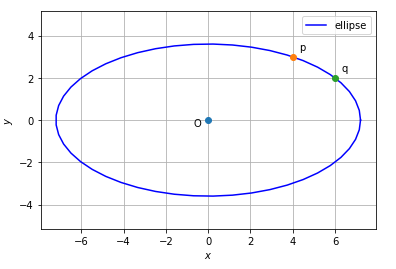
\includegraphics[width=\columnwidth]{ellipse(1).PNG}
\caption{Plot of standard ellipse}
\label{Plot of standard ellipse}
\end{figure}

The center and axes of the ellipse is given as
\begin{align}
\vec{c} = \vec{0};
\frac{1}{\sqrt{\lambda_1}}  = \sqrt{52},
\frac{1}{\sqrt{\lambda_2}} =\sqrt{13}.
\end{align}
Now let us consider the case when the ellipse is not in the standard form then we have the center to be $\vec{c}=\myvec{\beta\\0}$.The equation is given by:
\begin{align}
(\vec{x}-\vec{c})^{\top}\vec{D}(\vec{x}-\vec{c})=1\label{eq:14}
\end{align}
where $\vec{D}$ is a diagonal matrix.

$\because \vec{p}, \vec{q}$ satisfy \eqref{eq:14}, we have
\begin{align}
\label{eq:ellipse_std_ab}
(\vec{p}-\vec{c})^{\top}\vec{D}(\vec{p}-\vec{c}) &= 1,
\\
(\vec{q}-\vec{c})^{\top}\vec{D}(\vec{q}-\vec{c}) &= 1,
\end{align}
which can be simplified as
\begin{align}
    2\brak{\vec{p}-\vec{q}}^{\top}\vec{D}\vec{c}=\vec{p}^{\top}\vec{D}\vec{p}-\vec{q}^{\top}\vec{D}\vec{q} \label{eq:4}
\end{align}
Using the identity,
\begin{align}
   (\vec{p}^{\top}-\vec{q}^{\top})\vec{D}(\vec{p}+\vec{q})
   =\vec{p}^{\top}\vec{D}\vec{p}-\vec{q}^{\top}\vec{D}\vec{q}
\end{align}
in the equation \eqref{eq:4}
\begin{align}
    2\brak{\vec{p}-\vec{q}}^{\top}\vec{D}\vec{c}=(\vec{p}-\vec{q})^{\top}\vec{D}(\vec{p}+\vec{q})\\
    \implies (\vec{p}-\vec{q})^{\top}\vec{D}(2\vec{c}-(\vec{p}+\vec{q}))
\end{align}
Thus $\vec{c}$ can be expressed in parametric form as
\begin{align}
\vec{c}=\frac{1}{2}((\vec{p}+\vec{q})+k\vec{D}^{-1}\vec{m}) \label{eq:7}
\end{align}
where,
\begin{align}
    (\vec{p}-\vec{q})^{\top}\vec{m}=0 \label{eq:6}
\end{align}

and $k$ is a constant.Substituting numerical values in \eqref{eq:6}, \begin{align}
    \vec{p}-\vec{q} = \myvec{-2 \\ 1} \implies \vec{m} = \myvec{-1 \\ -2}
\end{align}
and
\begin{align}
    \vec{p}+\vec{q} = \myvec{10 \\ 5}
\end{align}
substituting in \eqref{eq:7},we get
\begin{align}
 \myvec{\beta\\0}=\frac{1}{2}\brak{\myvec{10 \\ 5} + k\myvec{\frac{1}{\lambda_1}&0 \\ 0&\frac{1}{\lambda_2}}\myvec{-1 \\ -2}}
\end{align}
From the given information,the X-axis is the major axis.Hence,

\begin{align}
\frac{\lambda_2}{\lambda_1}>1 \implies
    \frac{20-4\beta}{5}>1\\
    \beta<3.75
\end{align}
The possible ellipse satisfying the above conditions are plotted below
\numberwithin{figure}{section}
\begin{figure}[!ht]
\centering
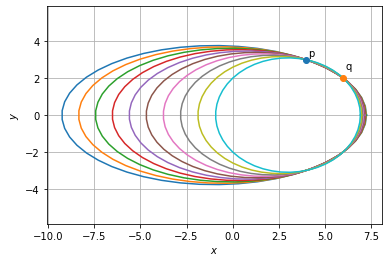
\includegraphics[width=\columnwidth]{Ellipse_(I).PNG}
\caption{Ellipses passing through the two points with X axis as major axis}
\label{fig:ellipses}	
\end{figure}
\end{document}
